\documentclass[10pt,a4paper]{article}
\usepackage{tocloft}
\usepackage{commons/course}  % همین کافیه؛ listings و xcolor داخلشه
\usepackage{booktabs}

% Define colors for syntax highlighting
\definecolor{keywordstyle}{rgb}{0.0, 0.4, 0.8} % A bluer shade
\definecolor{stringstyle}{rgb}{0.9, 0.17, 0.31} % amaranth
\definecolor{commentstyle}{rgb}{0.1, 0.6, 0.2} % green
\definecolor{numberstyle}{rgb}{0.4, 0.4, 0.4} % gray
\definecolor{backgroundcolor}{rgb}{0.94, 0.97, 1.0} % aliceblue

% Define the Python-like language for syntax highlighting
\lstdefinelanguage{PythonLike}{
	morekeywords={mov, add, sub, cmp, jmp , lw , addi,sw,bne},
	sensitive=false,
	morecomment=[l]{;},
	morestring=[b]",
}

% Set the style for Python-like code
\lstset{
	language=PythonLike,
	basicstyle=\ttfamily\small,
	keywordstyle=\color{keywordstyle},
	stringstyle=\color{stringstyle},
	commentstyle=\color{commentstyle},
	numbers=left,
	numberstyle=\tiny\color{numberstyle},
	stepnumber=1,
	numbersep=5pt,
	keepspaces=true,
	tabsize=4,
	showspaces=false,
	showstringspaces=false,
	showtabs=false,
	breaklines=true,
	breakatwhitespace=false,
	frame=single,
	backgroundcolor=\color{backgroundcolor},
}

\newlistof{listofproblems}{lop}{\normalsize فهرست مسائل}
\newcommand{\addproblem}[1]{\addcontentsline{lop}{listofproblems}{\protect\numberline{}#1}}


\begin{document}


\سربرگ{آزمایش دوم}{جمع‌کننده‌ی انتخاب رقم نقلی}{معین آعلی - ثمین اکبری}{استاد: دکتر حمید سربازی آزاد}

\subsubsection*{خلاصه}

در این آزمایش یک جمع‌کننده‌ی ۶ بیتی با تکنیک \lr{Carry Select} در نرم‌افزار \lr{Logisim} طراحی و پیاده‌سازی شده است. مدار به‌صورت سلسله‌مراتبی و از پایین به بالا ساخته شده: یک تمام‌جمع‌کننده‌ی ۱ بیتی (\lr{full\_adder})، که پایه‌ی ساخت یک جمع‌کننده‌ی ۲ بیتی \lr{ripple-carry} (\lr{adder2}) است، و در نهایت مدار اصلی (\lr{main}) با ترکیب پنج نمونه از این جمع‌کننده‌ی ۲ بیتی به‌همراه چهار قطعه‌ی آماده‌ی \lr{Multiplexer} از کتابخانه‌ی \lr{Logisim} ساخته شده است. این مدار \lr{Hybrid} از هر دو ابزار جمع‌کننده‌ی معمولی و مالتی‌پلکسر برای بهبود سرعت جمع نسبت به یک جمع‌کننده‌ی \lr{ripple-carry} صرف استفاده می‌کند.



\subsubsection*{ دیاگرام جمع‌کننده‌ی انتخاب رقم نقلی}
\begin{figure}[h]
  \centering
  
\includegraphics[width=0.95\textwidth]{figs/diagram.png}
\end{figure}


\subsubsection*{هدف آزمایش}

هدف از این آزمایش، آشنایی عملی با طراحی مدارهای \lr{Hybrid} (ترکیبی از جمع‌کننده و مدار انتخاب) به‌منظور بهبود سرعت عمل جمع است. برخلاف جمع باینری معمولی به‌روش \lr{ripple-carry} که در آن هر طبقه باید منتظر رقم نقلی طبقه‌ی قبل بماند، در تکنیک \lr{Carry Select} با محاسبه‌ی موازی و انتخاب بعدی، این انتظار تا حد زیادی حذف می‌شود. اهداف مشخص این آزمایش عبارت‌اند از:

\begin{itemize}
  \item پیاده‌سازی یک تمام‌جمع‌کننده‌ی ۱ بیتی (\lr{Full Adder}) با گیت‌های پایه.
  \item ساخت یک جمع‌کننده‌ی ۲ بیتی \lr{ripple-carry} از دو نمونه تمام‌جمع‌کننده.
  \item طراحی مدار جمع ۶ بیتی با تکنیک \lr{Carry Select}، با استفاده از جمع‌کننده‌های ۲ بیتی و قطعه‌ی آماده‌ی \lr{Multiplexer}.
  \item بررسی و درک مبادله‌ی سرعت در برابر سخت‌افزار در تکنیک \lr{Carry Select}.
\end{itemize}


\subsubsection*{چرا \lr{Carry Select}؟}

در یک جمع‌کننده‌ی \lr{ripple-carry} معمولی، هر طبقه باید منتظر رقم نقلی طبقه‌ی قبل بماند تا جمع خودش را شروع کند؛ تأخیر کل با تعداد بیت‌ها به‌صورت خطی رشد می‌کند. در \lr{Carry Select}، هر گروه از بیت‌ها را {دوبار و به‌موازات} جمع می‌زنیم -- یک‌بار با فرض $C_{in}=0$ و یک‌بار با فرض $C_{in}=1$ -- و وقتی رقم نقلی واقعی از طبقه‌ی قبل رسید، فقط با یک \lr{Multiplexer} جواب درست را انتخاب می‌کنیم. این کار محاسبه‌ی هر گروه را از انتظار برای رقم نقلی گروه قبلی آزاد می‌کند و تأخیر کلی مدار را کم می‌کند (به قیمت سخت‌افزار بیشتر، چون هر گروه به‌جز اولی باید دوبار جمع زده شود).


\subsubsection*{تمام‌جمع‌کننده‌ی ۱ بیتی}

\begin{center}
\begin{tabular}{@{}lll@{}}
\toprule
\textbf{پایه} & \textbf{جهت} & \textbf{پهنا} \\
\midrule
\lr{A}, \lr{B}, \lr{Cin} & ورودی & ۱ بیت \\
\lr{Sum}, \lr{Cout} & خروجی & ۱ بیت \\
\bottomrule
\end{tabular}
\end{center}

مدار با ۲ گیت \lr{XOR}، ۲ گیت \lr{AND} و ۱ گیت \lr{OR} ساخته شده است:

\begin{itemize}
    \item $X_1 = A \oplus B$ \\
    نیمه‌جمع، بدون در نظر گرفتن رقم نقلی ورودی.

    \item $P_1 = A \land B$ \\
    آیا از جمع $A$ و $B$ به‌تنهایی رقم نقلی تولید می‌شود؟

    \item $\mathrm{Sum} = X_1 \oplus C_{in}$ \\
    جمع نهایی سه ورودی.

    \item $P_2 = X_1 \land C_{in}$ \\
    آیا از جمع $X_1$ و $C_{in}$ رقم نقلی تولید می‌شود؟

    \item $\mathrm{Cout} = P_1 \lor P_2$ \\
    رقم نقلی خروجی نهایی.
\end{itemize}

\begin{LTR}
\begin{center}
\begin{tabular}{@{}ccc|cc@{}}
\toprule
A & B & Cin & Sum & Cout \\
\midrule
0 & 0 & 0 & 0 & 0\\
0 & 0 & 1 & 1 & 0\\
0 & 1 & 0 & 1 & 0\\
0 & 1 & 1 & 0 & 1\\
1 & 0 & 0 & 1 & 0\\
1 & 0 & 1 & 0 & 1\\
1 & 1 & 0 & 0 & 1\\
1 & 1 & 1 & 1 & 1\\
\bottomrule
\end{tabular}
\end{center}
\end{LTR}

{
\centering{
  
\includegraphics[width=0.8\textwidth]{figs/full-adder.png}
}
}



\subsubsection*{جمع‌کننده‌ی ۲ بیتی}

\begin{center}
\begin{tabular}{@{}lll@{}}
\toprule
\textbf{پایه} & \textbf{جهت} & \textbf{پهنا} \\
\midrule
\lr{A}, \lr{B} & ورودی & ۲ بیت \\
\lr{Cin} & ورودی & ۱ بیت \\
\lr{S} & خروجی & ۲ بیت \\
\lr{Cout} & خروجی & ۱ بیت \\
\bottomrule
\end{tabular}
\end{center}

ورودی‌های \lr{A} و \lr{B} با یک تفکیک‌کننده به بیت‌های تکی $A_0,A_1$ و $B_0,B_1$ شکسته می‌شوند و در زنجیره‌ای از ۲ تمام‌جمع‌کننده (\lr{FA0}, \lr{FA1}) به‌صورت \lr{ripple-carry} جمع زده می‌شوند:

\begin{center}
\begin{tabular}{@{}lllll@{}}
\toprule
\textbf{نمونه} & \textbf{بیت} & \textbf{ورودی‌ها} & \textbf{خروجی جمع} & \textbf{رقم نقلی} \\
\midrule
\lr{FA0} & ۰ (کم‌ارزش) & $A_0, B_0, C_{in}$ & $S_0$ & $C_1$ \\
\lr{FA1} & ۱ (پرارزش) & $A_1, B_1, C_1$ & $S_1$ & $\mathrm{Cout}$ \\
\bottomrule
\end{tabular}
\end{center}

بیت‌های $S_1S_0$ با یک تفکیک‌کننده‌ی ترکیبی دوباره به باس ۲ بیتی پایه‌ی خروجی \lr{S} وصل می‌شوند و رقم نقلی خروجی \lr{FA1} مستقیماً به پایه‌ی \lr{Cout} این مدار وصل است. این جمع‌کننده‌ی ۲ بیتی، بلوک سازنده‌ی اصلی مدار \lr{Carry Select} است و در مدار اصلی پنج بار نمونه‌سازی می‌شود.

{
\centering{
  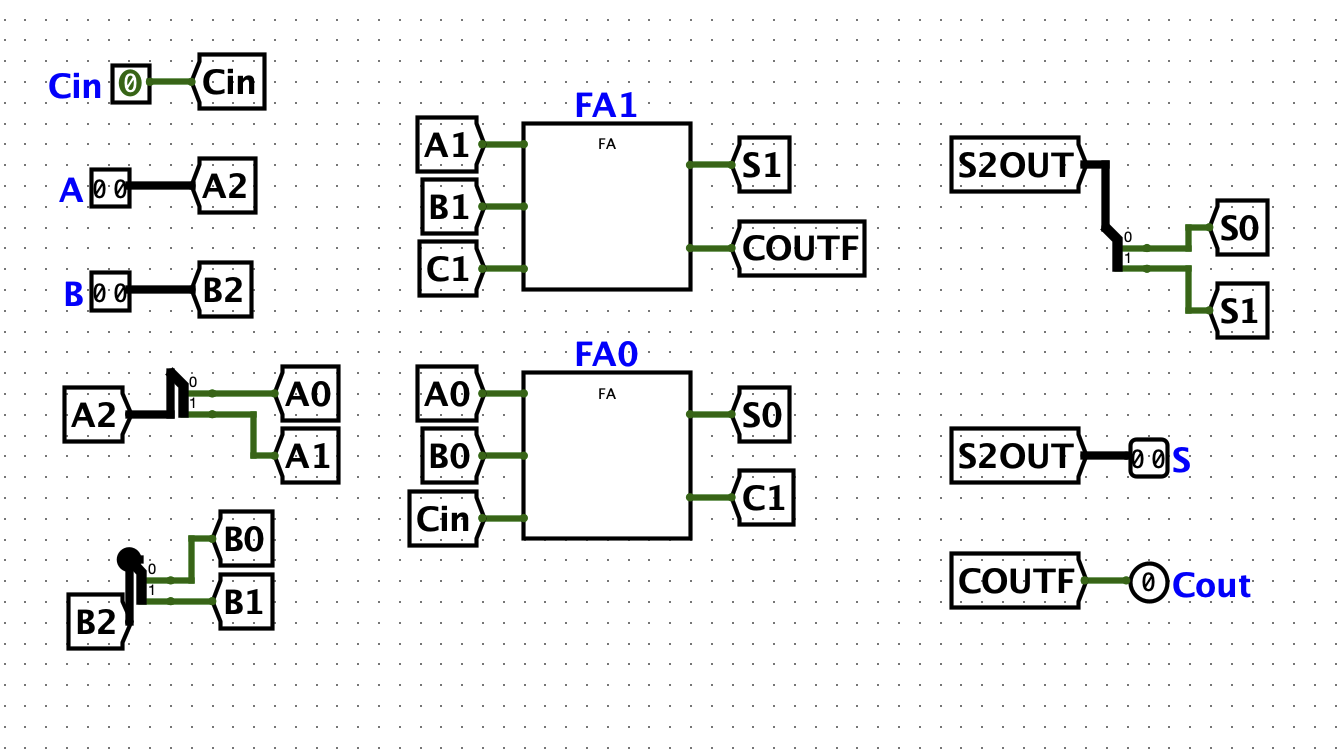
\includegraphics[width=0.9\textwidth]{figs/adder2.png}
}
}


\pagebreak


\subsubsection*{مدار اصلی}

\begin{center}
\begin{tabular}{@{}lll@{}}
\toprule
\textbf{پایه} & \textbf{جهت} & \textbf{پهنا} \\
\midrule
\lr{A}, \lr{B} & ورودی & ۶ بیت \\
\lr{Cin} & ورودی & ۱ بیت \\
\lr{S} & خروجی & ۶ بیت \\
\lr{Cout} & خروجی & ۱ بیت \\
\bottomrule
\end{tabular}
\end{center}

مدار به ۳ گروه ۲ بیتی تقسیم می‌شود. ابتدا \lr{A} و \lr{B} با یک تفکیک‌کننده‌ی ۶ به ۶ به بیت‌های تکی شکسته می‌شوند و بعد هر دو بیت هم‌گروه دوباره با یک تفکیک‌کننده‌ی ترکیبی به یک باس ۲ بیتی تبدیل می‌شوند تا وارد جمع‌کننده‌ی ۲ بیتی شوند:

\begin{center}
\begin{tabular}{@{}llll@{}}
\toprule
\textbf{گروه} & \textbf{بیت‌ها} & \textbf{باس} \lr{A} & \textbf{باس} \lr{B} \\
\midrule
گروه ۰ & ۱، ۰ (کم‌ارزش) & \lr{GA0} & \lr{GB0} \\
گروه ۱ & ۳، ۲ & \lr{GA1} & \lr{GB1} \\
گروه ۲ & ۵، ۴ (پرارزش) & \lr{GA2} & \lr{GB2} \\
\bottomrule
\end{tabular}
\end{center}

همچنین دو ثابت ساخته شده است: \lr{ZERO1} (ثابت ۰، برای فرض $C_{in}=0$) و \lr{ONE1} (ثابت ۱، برای فرض $C_{in}=1$).

\textbf{گروه ۰ (بیت‌های ۱،۰) -- بدون نیاز به انتخاب.}
چون این کم‌ارزش‌ترین گروه است، فقط یک رقم نقلی ورودی دارد (رقم نقلی واقعی \lr{Cin} مدار) و نیازی به \lr{Multiplexer} نیست:

\begin{center}
\begin{tabular}{@{}lllll@{}}
\toprule
\textbf{نمونه} & \lr{A} & \lr{B} & \lr{Cin} & \textbf{خروجی} \\
\midrule
\lr{AD0} & \lr{GA0} & \lr{GB0} & \lr{Cin} (واقعی) & $S_1S_0$, رقم نقلی $C_1$ \\
\bottomrule
\end{tabular}
\end{center}

رقم نقلی خروجی این طبقه، $C_1$، به‌عنوان {سیگنال انتخاب گروه بعدی} استفاده می‌شود.

\textbf{گروه ۱ (بیت‌های ۳،۲) -- انتخاب بر اساس $C_1$.}
جمع این گروه {دوبار و به‌موازات} با هر دو فرض ممکن برای رقم نقلی ورودی حساب می‌شود:

\begin{center}
\begin{tabular}{@{}lllll@{}}
\toprule
\textbf{نمونه} & \lr{A} & \lr{B} & \lr{Cin} & \textbf{خروجی} \\
\midrule
\lr{AD1\_0} (فرض بدون نقلی) & \lr{GA1} & \lr{GB1} & \lr{ZERO1} & $S_3S_2$ = \lr{SG1\_0}, رقم نقلی \lr{C3\_0} \\
\lr{AD1\_1} (فرض با نقلی) & \lr{GA1} & \lr{GB1} & \lr{ONE1} & $S_3S_2$ = \lr{SG1\_1}, رقم نقلی \lr{C3\_1} \\
\bottomrule
\end{tabular}
\end{center}

حالا با رسیدن $C_1$ واقعی، دو قطعه‌ی آماده‌ی \lr{Multiplexer} از کتابخانه‌ی \lr{Logisim} بین این دو جواب یکی را انتخاب می‌کنند:

\begin{center}
\begin{tabular}{@{}lllll@{}}
\toprule
\textbf{مالتی‌پلکسر} & \lr{D0} ($C_{in}=0$) & \lr{D1} ($C_{in}=1$) & \lr{Sel} & \textbf{خروجی} \lr{Y} \\
\midrule
\lr{MUXS1} (۲ بیت) & \lr{SG1\_0} & \lr{SG1\_1} & $C_1$ & $S_3, S_2$ نهایی \\
\lr{MUXC1} (۱ بیت) & \lr{C3\_0} & \lr{C3\_1} & $C_1$ & $C_3$ \\
\bottomrule
\end{tabular}
\end{center}

سیگنال $C_3$ (خروجی \lr{MUXC1}) هم رقم نقلی این گروه است، هم {سیگنال انتخاب گروه بعدی}.

\textbf{گروه ۲ (بیت‌های ۵،۴) -- انتخاب بر اساس $C_3$.}
دقیقاً همان الگوی گروه ۱، فقط با $C_3$ به‌جای $C_1$:

\begin{center}
\begin{tabular}{@{}lllll@{}}
\toprule
\textbf{نمونه} & \lr{A} & \lr{B} & \lr{Cin} & \textbf{خروجی} \\
\midrule
\lr{AD2\_0} & \lr{GA2} & \lr{GB2} & \lr{ZERO1} & $S_5S_4$ = \lr{SG2\_0}, رقم نقلی \lr{C5\_0} \\
\lr{AD2\_1} & \lr{GA2} & \lr{GB2} & \lr{ONE1} & $S_5S_4$ = \lr{SG2\_1}, رقم نقلی \lr{C5\_1} \\
\bottomrule
\end{tabular}
\end{center}

\begin{center}
\begin{tabular}{@{}lllll@{}}
\toprule
\textbf{مالتی‌پلکسر} & \lr{D0} ($C_{in}=0$) & \lr{D1} ($C_{in}=1$) & \lr{Sel} & \textbf{خروجی} \lr{Y} \\
\midrule
\lr{MUXS2} (۲ بیت) & \lr{SG2\_0} & \lr{SG2\_1} & $C_3$ & $S_5, S_4$ نهایی \\
\lr{MUXC2} (۱ بیت) & \lr{C5\_0} & \lr{C5\_1} & $C_3$ & \lr{COUTFINAL} \\
\bottomrule
\end{tabular}
\end{center}

سیگنال \lr{COUTFINAL} (خروجی \lr{MUXC2}) {رقم نقلی نهایی کل مدار} است و مستقیماً به پایه‌ی خروجی \lr{Cout} وصل می‌شود.

\textbf{مونتاژ نهایی.}
شش بیت $S_0, S_1, S_2, S_3, S_4, S_5$ با یک تفکیک‌کننده‌ی ۶ تایی دوباره به باس خروجی \lr{S} ترکیب می‌شوند.

\textbf{چرا این معماری سریع‌تر است؟}
چون \lr{AD1\_0}, \lr{AD1\_1}, \lr{AD2\_0}, \lr{AD2\_1} هیچ‌کدام منتظر رقم نقلی واقعی نمی‌مانند (هرکدام رقم نقلی ثابت خودشان را دارند)، همه‌ی این ۴ جمع‌کننده {می‌توانند کاملاً هم‌زمان و موازی با \lr{AD0}} شروع به محاسبه کنند. تنها چیزی که در انتها زمان می‌برد، عبور $C_1$ و سپس $C_3$ از میان یک لایه \lr{Multiplexer} است -- که خیلی سریع‌تر از عبور رقم نقلی واقعی از میان ۶ تمام‌جمع‌کننده‌ی پشت‌سرهم (مثل حالت \lr{ripple-carry} ساده) است.

\begin{center}
\begin{tabular}{@{}p{1cm}p{6.5cm}p{6.5cm}@{}}
\toprule
\textbf{مرحله} & \textbf{چه چیزی حساب می‌شود} & \textbf{منتظر چه سیگنالی است} \\
\midrule
۱ & \lr{AD0} جمع بیت‌های ۱،۰ را با \lr{Cin} واقعی حساب می‌کند و $C_1$ را تولید می‌کند & فقط \lr{Cin} واقعی مدار \\
۲ & \lr{AD1\_0} و \lr{AD1\_1} جمع بیت‌های ۳،۲ را برای هر دو حالت ممکن رقم نقلی از پیش حساب می‌کنند & هیچ‌چیز -- هم‌زمان با \lr{AD0} \\
۳ & \lr{MUXS1}/\lr{MUXC1} با $C_1$ بین دو جواب مرحله‌ی ۲ انتخاب می‌کنند و $C_3$ را می‌سازند & فقط رسیدن $C_1$ \\
۴ & \lr{AD2\_0} و \lr{AD2\_1} جمع بیت‌های ۵،۴ را برای هر دو حالت از پیش حساب می‌کنند & هیچ‌چیز \\
۵ & \lr{MUXS2}/\lr{MUXC2} با $C_3$ بین دو جواب مرحله‌ی ۴ انتخاب می‌کنند و \lr{Cout} نهایی را می‌سازند & فقط رسیدن $C_3$ \\
\bottomrule
\end{tabular}
\end{center}

{
\centering{
  
\includegraphics[width=1\textwidth]{figs/main.png}
}
}

\pagebreak

\subsubsection*{ نتایج تست}

هر سه مدار با بردار تست و از طریق خط فرمان \lr{Logisim} در حالت \lr{headless} تست شدند:

{
	\centering{

 		 
\includegraphics[width=0.7\textwidth]{figs/tests.png}

		 }
}


بردارهای تست داخل فایل‌های \lr{*.vec} قرار دارند و با اسکریپت \lr{run\_tests.sh} به‌صورت خودکار روی هر سه مدار اجرا می‌شوند.


\end{document}
